\documentclass{beamer} %[aspectratio=1610]

\usetheme{Darmstadt}
\usefonttheme[onlylarge]{structurebold}
\setbeamerfont*{frametitle}{size=\normalsize,series=\bfseries}
\setbeamertemplate{navigation symbols}{}

% Standard packages

\usepackage[english]{babel}
\usepackage[latin1]{inputenc}
\usepackage{times}
\usepackage[T1]{fontenc}
\usepackage{float}
\usepackage{graphicx}
\usepackage{subcaption}
\usepackage{ifthen}
\usepackage{minted}
\usepackage{verbatim}
%\usepackage{multimedia}
\usepackage{movie15}

% Setup TikZ
\usepackage{tikz}
\usetikzlibrary{arrows}
\tikzstyle{block}=[draw opacity=0.7,line width=1.4cm]


% Author, Title, etc.
\title[Pure functional programming in Agent-Based Simulation] 
{%
  Pure functional programming \\ in Agent-Based Simulation
}

\author[Thaler]
{
  Jonathan~Thaler
}

\institute[University of Nottingham, Nottingham, United Kingdom]
{
  University of Nottingham, Nottingham, United Kingdom
}

\date[Sandtable 21st June 2019]
{Sandtable 21st June 2019}

% The main document

\begin{document}

\begin{frame}
  \titlepage
\end{frame}

\section{Introduction}
\begin{frame}{The Metaphor}
\begin{itemize}
  \item "[..] object-oriented programming is a particularly natural development environment for Sugarscape specifically and artificial societies generally [..]" (Epstein et al 1996)
  
  \item "agents map naturally to objects" (North et al 2007)
\end{itemize}
\end{frame}

\begin{frame}{Outline}
\begin{itemize}
  %\item Defining Agent-Based Simulation (ABS)
  
  \item What is \textit{pure} Functional Programming (FP)?
  
  \item How can we do ABS + FP?  
  
  \item ABS + FP = ?
  
  \item Erlang = Future of ABS?
  
  \item Conclusions
\end{itemize}
\end{frame}

%\section{Agent-Based Simulation}
%\begin{frame}{Defining Agent-Based Simulation (ABS)}
%  \begin{block}{What is Agent-Based Simulation?}
%    Agent-Based Simulation is a methodology to \textbf{model} and \textbf{simulate} a system, where the \textbf{global behaviour} may be \textbf{unknown} but the behaviour and \textbf{interactions} of the \textbf{parts} making up the system \textbf{is known}. Those parts, called \textbf{agents}, are modelled and simulated, out of which then the aggregate \textbf{global behaviour} of the whole system \textbf{emerges}.
%  \end{block}
%\end{frame}
%
%\begin{frame}{Defining ABS cont'd}
%  \begin{block}{}
%    We informally assume the following about our agents \cite{macal_everything_2016, odell_objects_2002, siebers_introduction_2008, wooldridge_introduction_2009}:
%  \end{block}
%  
%  \begin{enumerate}
%    \item They are \textbf{uniquely addressable} entities with some \textbf{internal state} over which they have full, \textbf{exclusive control}.
%	\item They are \textbf{pro-active}, which means they can initiate actions on their own e.g. change their internal state, send messages, create new agents, terminate themselves.
%	\item They are situated in an \textbf{environment} and can \textbf{interact} with it.
%	\item They can \textbf{interact} with \textbf{other agents} situated in the same environment by means of \textbf{messaging}.
%  \end{enumerate}
%\end{frame}

\section{Functional programming}
\begin{frame}[fragile]{What is pure functional programming?}
  \begin{block}{Functions as first class citizens}
  	Passed as arguments, returned as values and assigned to variables.
  \end{block}
  
  \begin{block}{}
  \begin{minted}[fontsize=\normalsize]{Haskell}
  map :: (a -> b) -> [a] -> [b]
	
  const :: a -> (b -> a)
  const a = (\_ -> a)
  \end{minted}
  \end{block}
\end{frame}
 
\begin{frame}[fragile]{What is pure functional programming cont'd?}
  \begin{block}{Immutable data}
 	Variables can not change, functions return new copy. \\ Data-Flow oriented programming.
  \end{block}
  
  \begin{block}{}
  \begin{minted}[fontsize=\normalsize]{haskell}
  let x   = [1..10]
      x'  = drop 5 x
      x'' = x' ++ [10..20] 
  \end{minted}
  \end{block}
\end{frame}
 
\begin{frame}[fragile]{What is pure functional programming cont'd?}
  \begin{block}{Recursion}
 	To iterate over and change data. 
  \end{block}
  
  \begin{block}{}
  \begin{minted}[fontsize=\normalsize]{haskell}
  fact :: Int -> Int
  fact 0 = 1
  fact n = n * fact (n-1)
  \end{minted}
  \end{block}
\end{frame}
 
\begin{frame}[fragile]{What is pure functional programming cont'd?}
  \begin{block}{Declarative style}
  	Describe \textit{what} to compute instead of \textit{how}.
  \end{block}
  
  \begin{block}{}
  \begin{minted}[fontsize=\normalsize]{haskell}
  mean :: [Double] -> Double
  mean xs = sum xs / length xs
  \end{minted}
  \end{block}
\end{frame}
 
\begin{frame}[fragile]{What is pure functional programming cont'd?}
  \begin{block}{Explicit about Side-Effects}
  	Distinguish between side-effects of a function \textit{in its type}.
  \end{block}
  
  \begin{block}{}
  \begin{minted}[fontsize=\normalsize]{haskell}
  readFromFile      :: String -> IO String
  randomExponential :: Double -> Rand Double
  statefulAlgorithm :: State Int (Maybe Double)
  produceData       :: Writer [Double] ()
  \end{minted}
  \end{block}
\end{frame}

\section{ABS + FP}
\begin{frame}{How can we do ABS + FP?}
  \begin{block}{How can we represent an Agent, its local state and its interface?}
	We don't have objects and mutable state...
  \end{block}
  
  \begin{block}{How can we implement direct agent-to-agent interactions?}
	We don't have method calls and mutable state...
  \end{block}
  
  \begin{block}{How can we implement an environment and agent-to-environment interactions?}
	We don't have method calls and mutable state...
  \end{block}
  
  \begin{block}{Solution}
  	Functional Reactive Programming + \\ Monadic Stream Functions
  \end{block}
\end{frame}

\begin{frame}{Arrowized Functional Reactive Programming (AFRP)}
  \begin{itemize}
    \item Continuous- \& discrete-time systems in FP
 	\item Signal Function 
 	\item Events
 	\item Effects like random-numbers, global state, concurrency
 	\item \textit{Arrowized} FRP using the \textit{Dunai} library
  \end{itemize}
\end{frame}

\begin{frame}{Monadic Stream Functions (MSF)}
  \begin{block}{Process over time}
  \begin{flalign*}
	SF \, \alpha \, \beta \approx Signal \, \alpha \rightarrow Signal \, \beta \\
	Signal \, \alpha \approx Time \rightarrow \alpha 
  \end{flalign*}
  \end{block}
  
  \begin{block}{Agents as Signal Functions}
  \begin{itemize}
  	\item Clean interface (input / output)
  	\item Pro-activity by perceiving time
  	\item Closures + Continuations = very simple immutable objects
  \end{itemize}
  \end{block}
\end{frame}

\begin{frame}[fragile]{What are closures and continuations?}
\begin{block}{}
\begin{minted}[fontsize=\footnotesize]{haskell}
-- continuation type-definition
newtype Cont i o = Cont (i -> (o, Cont i o))

-- A continuation which sums up inputs.
-- It uses a closure to capture the input
adder :: Int -> Cont Int
adder x = Cont (\x' -> (x + x', adder (x + x')))
\end{minted}
\end{block}
\end{frame}

\begin{frame}{Agent-Based Spatial SIR Model}
  
\includegraphics[width=0.7\textwidth]{./fig/SIR_transitions.png}
  
  \begin{itemize}
    \item Population size $N = 1,000$
 	\item Contact rate $\beta = 5$
 	\item Infection probability $\gamma = 0.05$
 	\item Illness duration $\delta = 15$
 	\item 1 initially infected agent
 	\item On a 2D grid with Moore Neighbourhood
  \end{itemize}
\end{frame}

\begin{frame}{Agent-Based Spatial SIR Model Dynamics}
\begin{figure}
\begin{center}
	\begin{tabular}{c c}
		\begin{subfigure}[b]{0.4\textwidth}
			\centering
			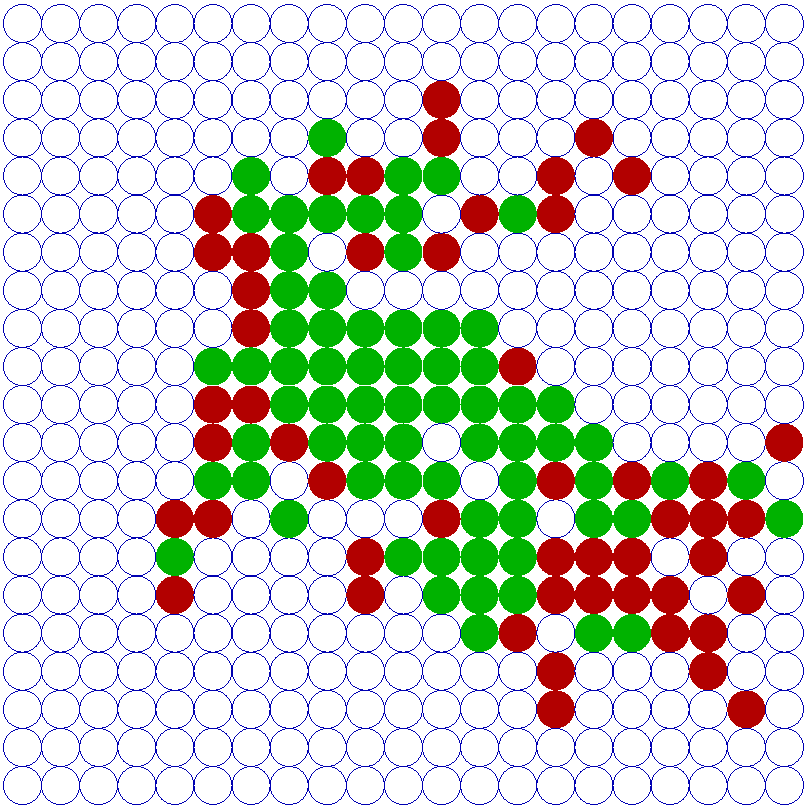
\includegraphics[width=1\textwidth, angle=0]{./fig/SIR_Dunai_dt001_environment.png}
			\caption{Environment at $t = 50$}
			\label{fig:sir_dunai_env}
		\end{subfigure}
    	
    	&
  
		\begin{subfigure}[b]{0.43\textwidth}
			\centering
			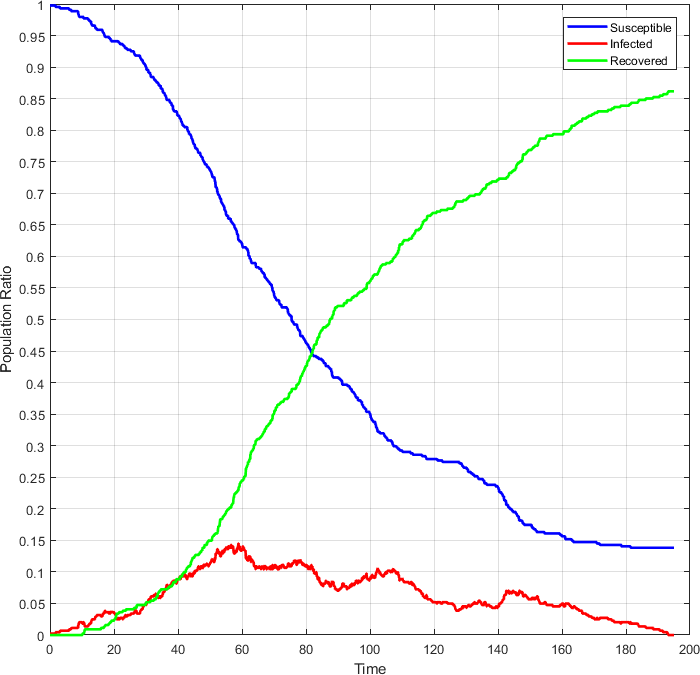
\includegraphics[width=1\textwidth, angle=0]{./fig/SIR_Dunai_dt001.png}
			\caption{Dynamics over time}
			\label{fig:sir_dunai_env_dynamics}
		\end{subfigure}
	\end{tabular}
\end{center}
\end{figure}
\end{frame}

\begin{frame}[fragile]{Recovered Agent}
\begin{block}{}
\begin{minted}[fontsize=\footnotesize]{haskell}
data SIRState    = Susceptible | Infected | Recovered

type Disc2dCoord = (Int, Int)
type SIREnv      = Array Disc2dCoord SIRState

type SIRAgent    = SF Rand SIREnv SIRState

recoveredAgent :: SIRAgent
recoveredAgent = arr (const Recovered) 
\end{minted}
\end{block}
\end{frame}

\begin{frame}[fragile]{Infected Agent}
\begin{block}{}
\begin{minted}[fontsize=\footnotesize]{haskell}
infectedAgent :: Double -> SIRAgent
infectedAgent delta
    = switch infected (const recoveredAgent)
  where
    infected :: SF Rand SIREnv (SIRState, Event ())
    infected = proc _ -> do
      recovered <- occasionally delta () -< ()
      if isEvent recovered
        then returnA -< (Recovered, Event ())
        else returnA -< (Infected, NoEvent)
\end{minted}
\end{block}
\end{frame}

\begin{frame}[fragile]{Susceptible Agent}
\begin{block}{}
\begin{minted}[fontsize=\footnotesize]{haskell}
susceptibleAgent coord beta gamma delta 
    = switch susceptible (const (infectedAgent delta))
  where
    susceptible :: SF Rand SIREnv (SIRState, Event ())
    susceptible = proc env -> do
      makeContact <- occasionally (1 / beta) () -< ()
      if isEvent makeContact
        then (do
          s <- randomNeighbour coord env -< as
          case s of
            Just Infected -> do
              i <- arrM_ (lift (randomBoolM gamma)) -< ()
              if i
                then returnA -< (Infected, Event ())
                else returnA -< (Susceptible, NoEvent)
            _       -> returnA -< (Susceptible, NoEvent))
        else returnA -< (Susceptible, NoEvent)
\end{minted}
\end{block}
\end{frame}

\section{ABS + FP = ?}
\begin{frame}{ABS + FP = Type Saftey}
	\begin{block}{Purity guarantees reproducibility at compile time}
    "... when the sequence of random numbers is specified ex ante the model is deterministic. Stated yet another way, model output is invariant from run to run when all aspects of the model are kept constant including the stream of random numbers." Epstein et al (1996)
    \end{block}
\end{frame}

\begin{frame}{ABS + FP = Enforce Update Semantics}
  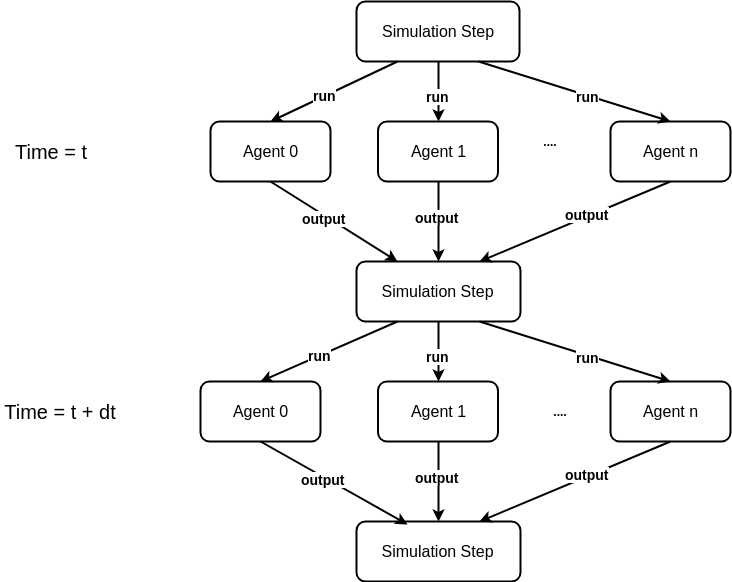
\includegraphics[width=0.7\textwidth]{./fig/parallel_strategy.png}
\end{frame}

\begin{frame}{ABS + FP = Software Transactional Memory}
  \begin{itemize}
  	\item Concurrency in ABS difficult.
	\item Synchronisation using locks.
  	\item $\Rightarrow$ error prone 
  	\item $\Rightarrow$ mixing of concurrency and model related code.
  	\item New approach in Haskell: Software Transactional Memory.
  \end{itemize}
\end{frame}

\begin{frame}{Software Transactional Memory (STM)}
  \begin{itemize}   	
  	\item Lock free concurrency.
  	\item Run STM actions concurrently and rollback / retry.
  	\item Haskell first language to implement in core.    
    \item Haskell type system guarantees retry-semantics.
  \end{itemize}
\end{frame}

\begin{frame}{Software Transactional Memory (STM)}
  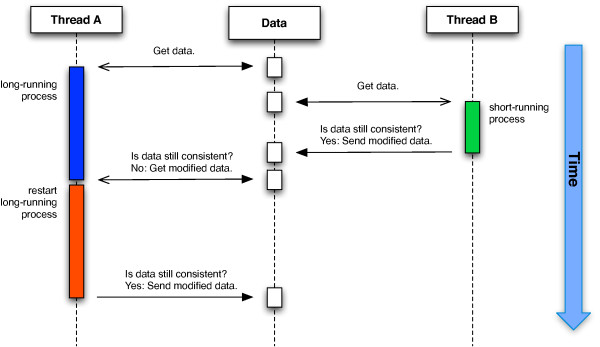
\includegraphics[width=0.9\textwidth]{./fig/stm.png}
\end{frame}

\begin{frame}{Software Transactional Memory (STM)}
  \begin{itemize}
  	\item Tremendous performance improvement.
  	\item No pollution of code with locking semantics.´
    \item Substantially outperforms lock-based implementation.
    \item STM semantics retain guarantees about non-determinism.
  \end{itemize}
\end{frame}

\begin{frame}{ABS + FP = Property-Based Testing}
  \begin{itemize}
    \item Express specifications directly in code.
    \item QuickCheck library generates random test-cases.
    \item Developer can express expected coverage.
    \item Random Property-Based Testing + Stochastic ABS = $\heartsuit \heartsuit \heartsuit$
  \end{itemize}
\end{frame}

\begin{frame}[fragile]{QuickCheck}
\begin{block}{List Properties}
\begin{minted}[fontsize=\footnotesize]{haskell}
-- the reverse of a reversed list is the original list
reverse_reverse :: [Int] -> Bool
reverse_reverse xs 
  = reverse (reverse xs) == xs

-- concatenation operator (++) is associative
append_associative :: [Int] -> [Int] -> [Int] -> Bool
append_associative xs ys zs 
  = (xs ++ ys) ++ zs == xs ++ (ys ++ zs)

-- reverse is distributive over concatenation (++)
reverse_distributive :: [Int] -> [Int] -> Bool
reverse_distributive xs ys 
  = reverse (xs ++ ys) == reverse xs ++ reverse ys
\end{minted}
\end{block}
\end{frame}

\begin{frame}[fragile]{QuickCheck cont'd}
\begin{block}{Running the tests...}
\begin{footnotesize}
\begin{verbatim}
+++ OK, passed 100 tests.
+++ OK, passed 100 tests.
*** Failed! Falsifiable (after 3 tests and 1 shrink):     
[1]
[0]
\end{verbatim}
\end{footnotesize}
\end{block}
\end{frame}

\begin{frame}[fragile]{QuickCheck cont'd}
\begin{block}{Labeling}
\begin{minted}[fontsize=\footnotesize]{haskell}
reverse_reverse_label :: [Int] -> Property
reverse_reverse_label xs  
  = label ("length of list is " ++ show (length xs)) 
          (reverse (reverse xs) == xs)
\end{minted}
\end{block}

\begin{block}{Running the tests...}
\begin{footnotesize}
\begin{verbatim}
+++ OK, passed 100 tests:
 5% length of list is 27
 5% length of list is 15
 5% length of list is 0
 4% length of list is 4
 4% length of list is 19
 ...
\end{verbatim}
\end{footnotesize}
\end{block}
\end{frame}

\begin{frame}[fragile]{QuickCheck cont'd}
\begin{block}{Coverage}
\begin{minted}[fontsize=\footnotesize]{haskell}
reverse_reverse_cover :: [Int] -> Property
reverse_reverse_cover xs  = checkCoverage 
  cover 15 (length xs >= 50) "length of list at least 50"
  (reverse (reverse xs) == xs)
\end{minted}
\end{block}

\begin{block}{Running the tests...}
\begin{footnotesize}
\begin{verbatim}
+++ OK, passed 12800 tests 
    (15.445% length of list at least 50).
\end{verbatim}
\end{footnotesize}
\end{block}
\end{frame}

\begin{frame}[fragile]{Property-Based Testing ABS example: SIR invariants}
\begin{minted}[fontsize=\footnotesize]{haskell}
prop_sir_invariants :: Positive Int    -- ^ contact rate
                    -> Probability     -- ^ infectivity (0,1)
                    -> Positive Double -- ^ illness duration
                    -> TimeRange       -- ^ duration
                    -> [SIRState]      -- ^ population
                    -> Property
prop_sir_invariants 
    (Positive cor) (P inf) (Positive ild) (T t) as  
  = property (do
    -- total agent count
    let n = length ss
    -- run the SIR simulation with a new RNG 
    ret <- genSimulationSIR ss cor inf ild t
    -- check invariants and return result
    return (sirInvariants n ret)
\end{minted}
\end{frame}

\begin{frame}[fragile]{Property-Based Testing ABS example: SIR invariants}
\begin{minted}[fontsize=\tiny]{haskell}
sirInvariants :: Int                    -- ^ N total number of agents
              -> [(Time,(Int,Int,Int))] -- ^ output each step: (Time, (S,I,R))
              -> Bool
sirInvariants n aos = timeInc && aConst && susDec && recInc && infInv
  where
    (ts, sirs)  = unzip aos
    (ss, _, rs) = unzip3 sirs

    -- 1. time is monotonic increasing
    timeInc = allPairs (<=) ts
    -- 2. number of agents N stays constant in each step
    aConst = all agentCountInv sirs
    -- 3. number of susceptible S is monotonic decreasing
    susDec = allPairs (>=) ss
    -- 4. number of recovered R is monotonic increasing
    recInc = allPairs (<=) rs
    -- 5. number of infected I = N - (S + R)
    infInv = all infectedInv sirs

    agentCountInv :: (Int,Int,Int) -> Bool
    agentCountInv (s,i,r) = s + i + r == n

    infectedInv :: (Int,Int,Int) -> Bool
    infectedInv (s,i,r) = i == n - (s + r)

    allPairs :: (Ord a, Num a) => (a -> a -> Bool) -> [a] -> Bool
    allPairs f xs = all (uncurry f) (pairs xs)

    pairs :: [a] -> [(a,a)]
    pairs xs = zip xs (tail xs)
\end{minted}
\end{frame}

\begin{frame}{Property-Based Testing Conclusion}
  \begin{itemize}
    \item Matching the constructive and exploratory nature of ABS.
    \item Test agent specification.
    \item Test simulation invariants.
    \item Exploratory models: hypotheses tests about dynamics.
    \item Explanatory models: validate against formal specification.
  \end{itemize}
\end{frame}

\section{Drawbacks}

\begin{frame}{ABS + FP = Drawbacks!}
  \begin{itemize}
    \item Direct bi-directional / sync Agent-interactions are \textit{very} cumbersome.
    \item STM not applicable to direct agent-interactions.
    \item MSFs can become \textit{terribly} slow!
    \item Steep learning curve: learning Haskell \textit{is} hard.
    \item (Good) Haskell programmers are a \textit{very} scarce resource.
    \item Strong, static type-system burden, sometimes want to be more dynamic.
  \end{itemize}
  
  \begin{block}{Is (pure) functional ABS a dead end?}
    On the contrary, it is just the beginning... enter Erlang!
  \end{block}
\end{frame}

\section{Erlang}

\begin{frame}{Erlang = Future of ABS?}
  \begin{itemize}
    \item Functional language; dynamically strongly typed; \textit{not} pure.
    \item Actor Model: message-based concurrency, shared-nothing semantics.
    \item Extremely robust and mature: 1.7 million lines of code in Eriksson telecom switch, 2 hours downtime in 40 years.
    \item Property-based testing: detect races and deadlocks.
    \item STM behaviour: can be emulated or use Erlangs Mnesia.
    %\item emulate oo: encapsulation (obviously), polymorphism (same interface, different behaviour), basiclly like a immutable, single method object, which transitions into a new object upon reception of a message, sync method-call possible (send and receive)
    \item Philosophy: fail fast! % seems to work as proven in highly complex industry 
  \end{itemize}
\end{frame}

\begin{frame}{Erlang + ABS}
  \begin{itemize}
  	\item Prototypes (SIR, Sugarscape) look promising.
  	\item Performance is promising. %substantially faster than pure functional Haskell approach, still slower than a sequential java approach BUT it should scale much better to large number of agents 
    \item Maps naturally to models with complex agent-interactions with the need to scale up.
    \item Easy emulation of data-parallelism. % (though not statically guaranteed).
    \item Use Process Calculi (CPS, CCS, pi-calculus) for specification and algebraic reasoning.
  \end{itemize}
  
  \begin{block}{The Future?}
Agent-interaction heavy model with huge populations of computationally expensive agents, needing a distributed always online approach, which can be updated while simulation is running (e.g. introduce new agents).
  \end{block}
\end{frame}

\section{Conclusions}

\begin{frame}{Conclusion}
\begin{block}{Have we done ABS implementation wrong?}
No, but we missed out on a lot of potential!
\end{block}

\begin{block}{I hypothesise that Erlang could be the future of ABS}
But... who is going to take the risk?
\end{block}
\end{frame}

\begin{frame}{}
  \begin{center}
  Thank You!
  \end{center}
\end{frame}

\bibliographystyle{acm}
\bibliography{../../writing/references/phdReferences.bib}

\end{document}